\documentclass[../main.tex]{subfiles}

\graphicspath{{\subfix{../imgs/}}}

\begin{document}

\section{Task 3.3}

Create two modules that realize a producer and a consumer thread. The modules should be connected together using a \textbf{sc\_fifo} channel. Use the structure of a TCP package to simulate the data transmitted over the transmission (fifo) channel. The producer transmits a new TCP package with a random interval between 2-10 ms. The consumer thread must print the simulation time and sequence number each time a new TCP package is received. Use the TCP Header structure as described below with a total package size of 512 bytes. Inspiration can be found in the \textbf{FifoFilter} (Fork.h, when adding two consumers) example project.


\begin{figure}[h]
    \centering
    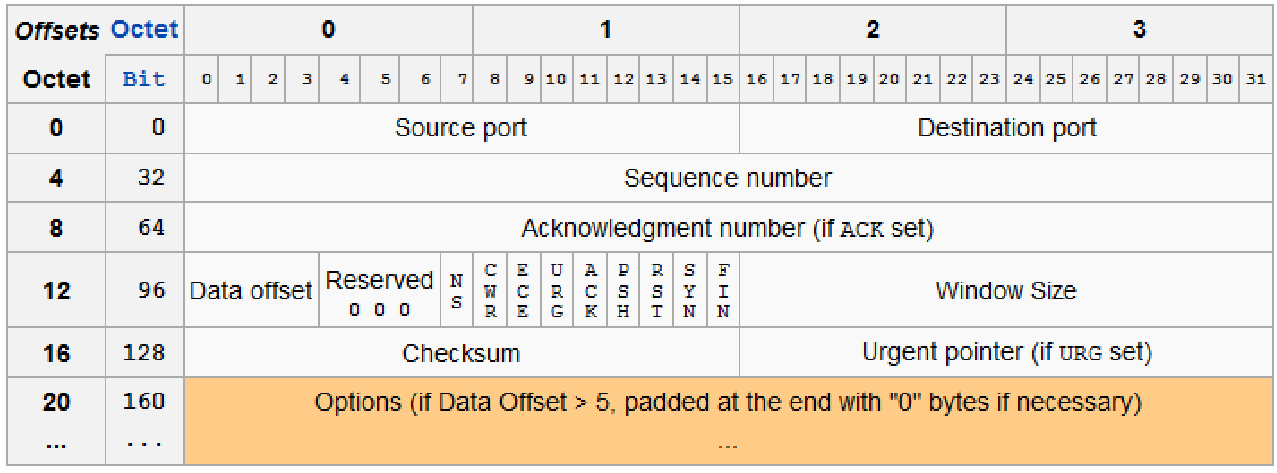
\includegraphics[width=0.9\textwidth]{task_3_3.png}
    \caption{TCP header structure.}
    \label{fig:tcp}
\end{figure}

Extend your model to have two fifo channels and consumers receiving TCP packes on port 1 and 2. The producer must be rewritten to connect to more ports.

\subsection*{Solution}

\end{document}

